\documentclass[11pt,a4paper]{article}
\usepackage{graphicx}
\graphicspath{ {images/} }
\usepackage{url}
\usepackage{natbib}
\usepackage[rightcaption]{sidecap}
%\usepackage{transparent}
%\usepackage{xcolor}
\usepackage{relsize}
\usepackage{amsmath}
\usepackage{amsfonts}
\usepackage[margin=2cm]{geometry}
\usepackage{fancyhdr}
\usepackage{enumitem}
\pagestyle{fancy}
\usepackage{float}
\usepackage{cancel}
\usepackage{subfig}
\usepackage{multirow}
\usepackage{varioref}
\usepackage{mathtools}
\usepackage[utf8]{inputenc}

\numberwithin{equation}{subsection}

\newtagform{fn}{(}{)\footnotemark}

\pagenumbering{arabic}


\fancyhf{}               
\fancyhead[L]{\rightmark}   
\fancyhead[C]{\thepage}
\fancyhead[R]{Personal code: fzn106}  

\begin{document}
In order to asses the derived method I will consider the following trials. Each of them will have the flowing properties. 
\subsection{Trial 1: Patterns in Average runs.}
Patterns in e derived algorithm will not show in individual solutions, because of that we will look at the averages of 5 solutions each with a different randomized set of errors $\xi_i$ an therefore different values $\tilde{y}_i$.\\
\\
TABLE\\
\\
We can notice a concrete pattern in these values. For the solutions of the derived method, as the standard deviation $\sigma$ of error $\xi$ increases (i.e. the error values spread to a larger range.) we also see an increase in both the expected error proposed by the derived method and the factual error it made. This is not surprising as this is the expected result of the increase of $\sigma$ of $\xi$. There is also nothing special in that LAD is generally better than the derived method at giving the parameters of the function, other than the case where $\sigma = 1.0$, there (I presume) some values $\xi$ were slanted to be large in the positive sign, skewing LAD's solution up. The reason why the derived method gives a better result there is because it is less responsive to such large peaks in $\xi$ as it weighs them the same way as the rest of the values of $\xi$. This will be important in the second trial.

\subsection{Trial 2: Comparison of derived method vs. LSM}

Clearly, the derived method will have advantage over the LSM if the condition $E(\xi)=0$ is not fulfilled. To show this, I calculated 5 algorithm trails using the same description as stated above with $\sigma=0.3$ while using the proximity function used in LSM, but with one big difference. Two of the largest values of $\xi$ are increased by a factor of 5. Table 3 illustrates the solutions given by the derived method and LSM with these conditions in mind.\\
\\
TABLE\\
\\
The factual errors made by the derived method is tens times smaller than the ones made by LSM. This is semi-misleading, as the LSM proximity (factual error in $c_1=(\dot{c_1}-c_1)^2$ or the difference between true and approximated value all squared.) function was used to calculate the factual error for both methods, and as the difference between the true and approximated components by the derived method are themselves quite small and less than 1, their squares will resemble the factual error displayed in the table.\\
\\
\begin{figure}[h!]
\caption{Graph of trial number 4 from Table 3. LSM's solution is definitively worse.}
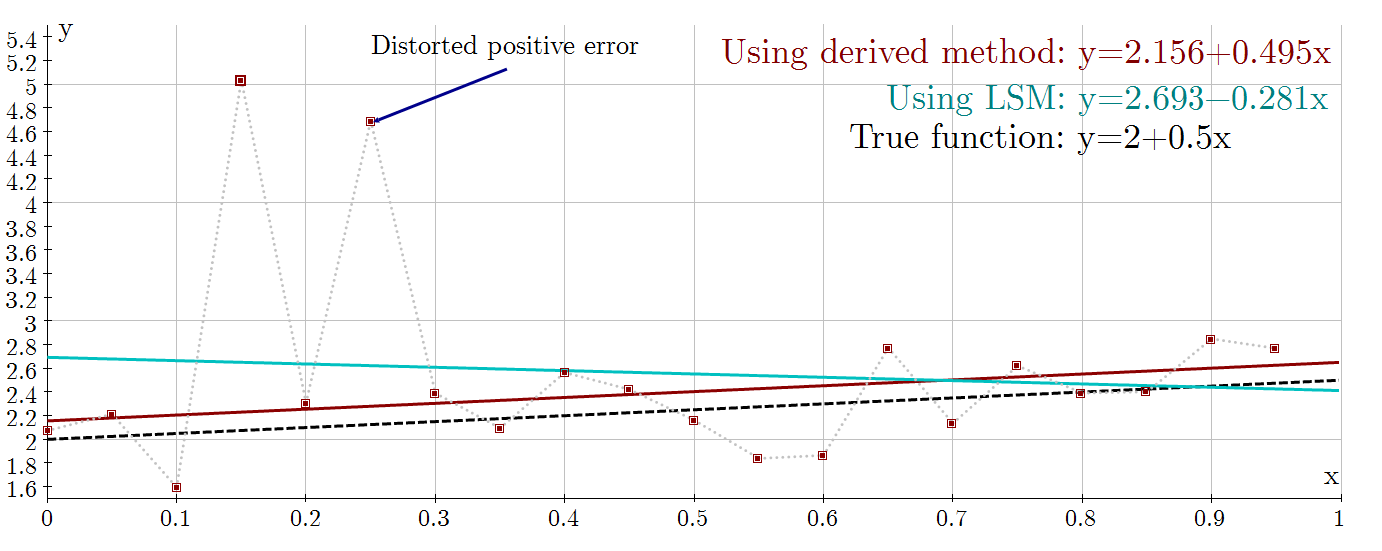
\includegraphics[scale=0.35]{updated/table-2}
\centering
\end{figure}
To visually represent in what ways the derived method is superior to LSM, I graphed the 4th trail from the previous table. Here, due to the two enlarged values of errors $\xi$ (which are weighted more by the LSM) LSM provides a solution linear function with a negative gradient, completely misrepresenting the true function that has a positive gradient. 
\end{document}
